\documentclass[12pt,a4paper]{article}

\usepackage[T1]{fontenc}
\usepackage[utf8]{inputenc}
\usepackage[margin=2.5cm]{geometry}
\usepackage{setspace}
\usepackage[round,authoryear]{natbib}
\usepackage[hidelinks]{hyperref}
\usepackage{graphicx}
\usepackage{float}
\usepackage{tikz}
\usetikzlibrary{arrows.meta,positioning}
\usepackage{pgfgantt}
\usepackage{tabularx}
\usepackage{booktabs}
\usepackage{caption} % Required for \captionof
\newcolumntype{L}{>{\raggedright\arraybackslash}X}

\begin{document}
\pagenumbering{gobble}

% -------------------------------------------------
% Title page
% -------------------------------------------------

\begin{titlepage}
\centering
\vspace*{2cm}

{\large University of Liverpool\par}
{\large School of Computer Science and Informatics\par}

\vspace{1.2cm}

{\normalsize COMP702 --- MSc Dissertation\par}
{\normalsize Specification and Design Proposal (CA1)\par}

\vspace{3cm}

{\LARGE\bfseries Multi-Agent Debate Frameworks\par}
\vspace{0.3cm}
{\LARGE\bfseries for Enhanced Truthfulness\par}

\vspace{3cm}

{\large Dmytro Honchar\par}
\vspace{0.2cm}
{Student ID: 201951718\par}
{Username: sgdhonch\par}

\vspace{1.2cm}

{\large Supervisor: Meng Fang\par}
{\large Second Marker: Katie Atkinson\par}

\vfill

{\large Submission date: \today\par}

\end{titlepage}
\pagenumbering{arabic}

% -------------------------------------------------
% Statement of ethical compliance
% -------------------------------------------------

\section{Statement of Ethical Compliance}
\label{sec:ethical-compliance}

\noindent
\textbf{Data Category: A}\\
\textbf{Participant Category: 0}

\vspace{0.5cm}

\noindent
I confirm that I have read the relevant ethical guidelines and will follow them
throughout this project.

\vspace{0.3cm}

\noindent
The research uses one publicly available benchmark dataset, MMLU-Pro. It is a
set of multiple-choice questions with answer labels collected for research
evaluation. It contains no personal, sensitive or identifiable data, and it
includes no clinical records. I will use the dataset under its published
licence terms. The remaining experimental data will consist of model prompts
and the responses returned by the models.

\vspace{0.3cm}

\noindent
The project does not involve human participants. I will not recruit, interview,
survey or observe anyone, and no usability feedback will be collected as
research data. The replay interface is only for inspecting and presenting
experimental results. If this changes, I will submit an ethics amendment before
any participants are involved.

\vspace{1.5cm}

\noindent
\textbf{Name:} Dmytro Honchar

\vspace{0.5cm}

\noindent
\textbf{Student ID:} 201951718

\vspace{0.5cm}

\noindent
\textbf{Signature:} Dmytro Honchar

\vspace{0.5cm}

\noindent
\textbf{Date:} \today

% -------------------------------------------------
% Generative AI declaration
% -------------------------------------------------

\section*{Generative AI Use Declaration}


Generative AI tools (ChatGPT Sol 5.6 (OpenAI), Claude Opus 5 (Anthropic)) were used to support project planning,
methodological discussion, software implementation, debugging, testing,
document revision and language editing. I reviewed and tested all
AI-assisted contributions and checked factual, methodological and
literature-based claims against the original sources. The experimental
responses were generated only by the five models specified in this project
through OpenRouter. The coding assistants were not experimental agents and
did not alter benchmark answer labels or manually create recorded results.
The final project decisions are my own, and I take responsibility for the
submitted work.

% -------------------------------------------------
% Project description
% -------------------------------------------------

\section{Project Description}

This project will build an orchestrated multi-agent debate system to test
whether communication between large language model (LLM) agents improves answer
accuracy, leaves it unchanged or makes it worse, and whether any improvement
justifies the additional computational cost. The evaluation will use MMLU-Pro,
a multi-subject multiple-choice benchmark with reference answer labels and up
to ten answer options. For this project, truthfulness is operationally defined
as correctness against the MMLU-Pro answer labels.

The system will use five agents from different open-weight model families:
Llama, Qwen, Mistral, DeepSeek and Gemma. In round one, they will answer the
same question independently. In round two, each agent will receive the original
question, its own round-one response if it was valid, and the available valid
responses produced by the other four agents with agent, model and provider
identities removed.

The group vote after each round will be recorded for evaluation. The round-one
group vote will not be shown to the agents before round two.

A group answer after either round will require at least three matching answers
from the five configured agents. Failed responses will cast no vote and will
not reduce this threshold. If no answer reaches three votes, no group answer
will be recorded.

% -------------------------------------------------
% Aim and requirements
% -------------------------------------------------

\section{Aim and Requirements}

\subsection{The Main Aim}

The main aim is to determine how much of any accuracy gain in a five-agent LLM system comes from communication between agents, and whether aggregating independent answers through majority voting achieves the same accuracy without debate. The project will evaluate these effects using the same questions, agents, model settings, round-specific prompts and voting rule, while also considering computational cost.


\subsection{Research Question}


    Does cross-model debate improve answer accuracy beyond what is already achieved through majority voting?


\subsection{Requirements}

\subsubsection*{Essential requirements}

\begin{itemize}
    \item The system must run debates between five LLM agents selected through
    a configurable model setup and accessed through the OpenRouter API.

    \item In round one, each agent must answer independently, returning an
    explanation and one selected answer. In round two, each agent must receive
    its own valid round-one response and the available valid responses of the
    other agents with their identities removed, and then return a revised
    explanation and answer.

    \item The system must calculate a majority vote after round one, before any
    communication, and again after round two. The first vote must not be shown
    to the agents. A majority always requires at least three matching answers
    from the five configured agents. Failed responses cast no vote and do not
    reduce this threshold.

    \item The system must log every agent response in every round, together with
    its question identifier, parse status, both group votes and the final group
    result. Correct answers must remain in a separate answer-key file and must
    be joined with the experimental results only during evaluation.

    \item The evaluation must report each agent's round-one accuracy and the
    group accuracy after both votes. It must also report consensus, failures,
    answer changes, token usage, estimated cost and latency.

    \item A replay interface must allow one debate to be inspected round by
    round, showing each agent's response and how the group result was reached.

    \item The dataset pipeline must produce a fixed sample of MMLU-Pro questions
    that is reused across all experimental runs, with the answer key stored
    separately from the questions sent to the models.
\end{itemize}

\subsubsection*{Desirable requirements, if time permits}

\begin{itemize}
    \item An additional debate round for questions without a majority after
    round two, giving agents one further chance to reach consensus.

    \item Results broken down by MMLU-Pro subject category.
\end{itemize}

% -------------------------------------------------
% Key literature and background reading
% -------------------------------------------------

\section{Key Literature and Background Reading}

\subsection{Multi-agent debate as a technique}

Large language models are commonly used through a single prompt and response,
so the result depends on one reasoning path and one sampled output. Multi-agent
systems instead combine several model responses. Self-consistency selects the
answer that appears most often across several solutions from one model
\citep{wang2023selfconsistency}. In multi-agent debate (MAD), several agents
solve the same question independently and then exchange their answers and
reasoning, allowing them to reconsider their initial positions.

\citet{du2024multiagent} introduced a debate method in which several instances
of the same model answered a question, compared their reasoning, and revised
their answers over multiple rounds. It improved performance on mathematics,
chess and factuality tasks. When different models are used, they may also
contribute different knowledge and problem-solving abilities.

\subsection{Evidence from previous studies}

ReConcile used ChatGPT, Bard and Claude~2 with confidence-weighted voting
\citep{chen2024reconcile}. On StrategyQA, the mixed-model group achieved 79.0\%
accuracy compared with 72.2\% for three ChatGPT agents, and its accuracy rose
from 74.3\% before discussion to 79.0\% afterwards. However, the models also had
different initial capabilities, so the source of the improvement is unclear.

\citet{smit2024mad} compared debate with simpler ways of combining model
answers. Debate did not consistently perform better, despite requiring more
model calls and time, and its results were sensitive to prompt design.

\citet{choi2025debate} examined two separate parts of MAD. First, the agents
answered independently, and the group answer was selected by majority vote. The
agents then discussed the question and were allowed to change their answers.
The study found that most of the improvement came from majority voting, while
the discussion itself added little. On one arithmetic task, Qwen2.5-7B achieved
99\% with majority voting, but this fell to 76\% after two debate rounds and
67\% after three and five rounds.

\citet{zhang2025heterogeneity} found that randomly mixing GPT-4o-mini and
Llama~3.1~70B improved the final accuracy of five MAD systems. However, agents
did not keep fixed model identities, and the mixed group's vote was not measured
before discussion. The study therefore does not separate the effects of mixing
the initial answers, voting and discussion.

M3MAD-Bench tested nine models across thirteen datasets and likewise found that
debate did not consistently improve accuracy \citep{li2026m3mad}. Mixed groups
could outperform the weakest single-model groups but usually not the strongest,
while additional rounds required more tokens and time and could move answers in
either direction.

\subsection{Research gap}

Studies use different models, benchmarks, prompts, agent counts, debate rounds
and aggregation methods. They do not always separate individual model ability,
majority voting and discussion. This project therefore checks whether debate
between cross-model agents improves accuracy and whether voting alone achieves
the same result.

\subsection{Project response and evaluation setting}

The project measures each model's initial accuracy, the majority vote before
discussion and the final vote after discussion. The same frozen questions,
agents, model settings, round-specific prompt versions and voting rule are used
throughout, and each agent keeps its assigned model. Answer changes, consensus,
token usage, cost and response time are also recorded. MMLU-Pro provides fixed answer labels across fourteen subjects and up
to ten options, allowing automatic scoring while reducing random agreement
\citep{wang2024mmlupro}.
The system uses two rounds, with only one round of communication, because
previous work shows that further debate rounds do not always improve results
and can sometimes reduce accuracy \citep{choi2025debate,li2026m3mad}.
% -------------------------------------------------
% Preliminary work
% -------------------------------------------------

\section{Preliminary Work}
\label{sec:preliminary}

The repository contains local copies of the MMLU-Pro test and validation
datasets. The exact dataset version and file checksums are recorded to confirm
that the files have not changed. Python code gives each question a stable ID and
checks its text, answer options and correct label. It rejected 15 questions with
duplicate answer options: one test question and 14 validation questions.

A repeatable sampling process was implemented using a fixed random seed. The
code created 300 experimental questions and 20 separate pilot questions. Both sets were sampled from the MMLU-Pro test split only. The
two sets do not overlap and cover all 14 subjects. Files shown to the models do
not contain the correct answers, which are stored separately. The freezing code
also prevents accidental overwriting. Sixteen automated data-preparation tests
pass, including
tests for repeatable sampling, non-overlapping sets, checksums and prevention of
answer leakage.

The frozen data pipeline is complete. The five-model configuration,
OpenRouter client, prompt construction, parsing, caching, result storage,
voting and both debate rounds are implemented and covered by automated
tests. Round one and one complete two-round debate have been verified with
a small number of live API calls. The formal 20-question pilot and the
300-question main experiment have not yet been run.

\section{Development and Implementation Summary}
\label{sec:implementation}

The system will follow a fixed pipeline that separates dataset processing,
model configuration, debate orchestration, result storage and evaluation. This
helps to keep the experiment reproducible and prevents correct answers from
being sent to the models.

\begin{enumerate}

    \item \textbf{Dataset preparation.}
    The validated dataset contains 300 main questions and 20 separate pilot
    questions, with the answer keys stored separately.

    \item \textbf{Experiment configuration.}
    Configuration files will define the model, provider and maximum output length for each agent. All models will use temperature 0 and top-p 1.0 to reduce variation between repeated requests. Each model will use a fixed provider, and OpenRouter will not be allowed to switch providers automatically. After the pilot, these settings will be fixed for the main experiment.

    \item \textbf{Prompt construction.}
    Each round will use a fixed, versioned prompt. Round one requests an
    independent explanation and answer. Round two includes the agent's own valid
    previous response and the available valid responses of the other agents,
    with agent, model and provider identities removed.

    \item \textbf{Model-calling layer.}
    A shared OpenRouter interface will call every model and record the model,
    provider, token usage, cost, latency and API status. Temporary failures will
    be retried once. Persistent failures will be recorded and will cast no vote.

    \item \textbf{Caching and response processing.}
    A cache will avoid repeated calls. Responses will be saved as received, and
    one parser will extract answers and record failures.

    \item \textbf{Round-one execution.}
    Five agents will answer independently before the first majority vote.

    \item \textbf{Round-two debate.}
    Each agent will receive its own valid round-one response and the available
    valid responses of the other agents with their identities removed, and will
    then reconsider its answer. The first group vote will be recorded for comparison but will not be included in the round-two prompt.

    \item \textbf{Voting and result storage.}
    The second vote requires three matching answers; otherwise, it records no
    consensus. Responses, votes and metadata will be stored in SQLite.

    \item \textbf{Pilot run.}
    The 20 pilot questions will test both rounds, parsing, storage, prompt
    length, cost and time before the main run (Section~\ref{sec:testing}).

    \item \textbf{Evaluation.}
    Individual round-one accuracy and both group votes will be compared with
    answer changes, consensus, cost and latency.

    \item \textbf{Replay interface.}
    A Streamlit page will display completed debates without calling any model.

\end{enumerate}

The implementation will use \textbf{Python}, \textbf{OpenRouter}, separate
\textbf{SQLite} databases for cached responses and results, \textbf{YAML}
configuration, \textbf{pytest} and \textbf{Streamlit}.

The high-level architecture is illustrated in Figure~\ref{fig:pipeline}.

\begin{figure}[htbp]
    \centering
    \resizebox{\textwidth}{!}{%
    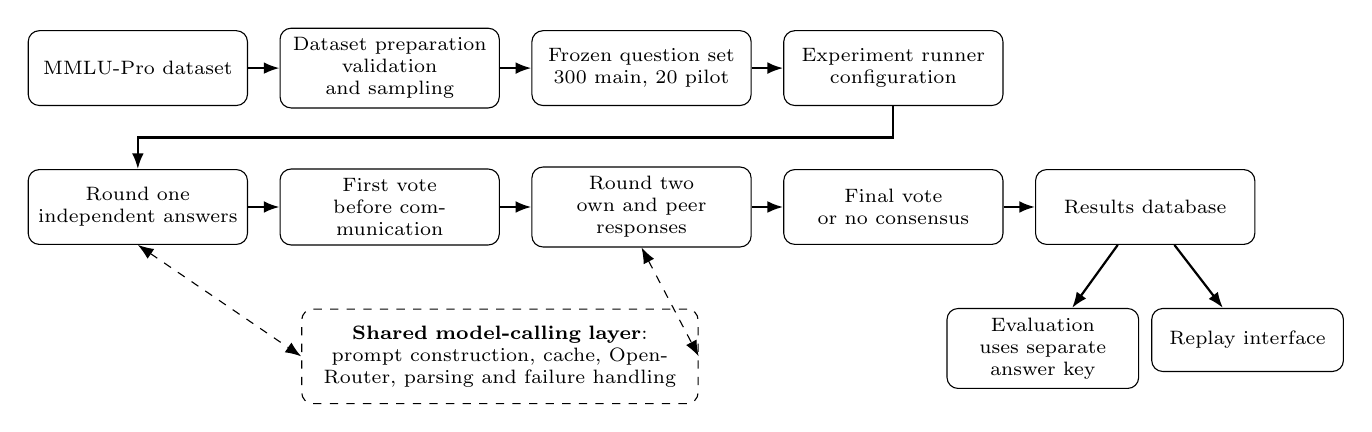
\begin{tikzpicture}[
        box/.style={
            draw,
            rounded corners,
            align=center,
            text width=2.55cm,
            minimum height=0.95cm,
            font=\scriptsize
        },
        small/.style={
            draw,
            rounded corners,
            align=center,
            text width=2.2cm,
            minimum height=0.8cm,
            font=\scriptsize
        },
        service/.style={
            draw,
            dashed,
            rounded corners,
            align=center,
            text width=4.8cm,
            minimum height=1.2cm,
            font=\scriptsize
        },
        flow/.style={-{Latex[length=2mm]},thick},
        call/.style={{Latex[length=2mm]}-{Latex[length=2mm]},dashed},
        node distance=4mm
    ]

        \node[box] (dataset) {MMLU-Pro dataset};
        \node[box, right=of dataset]
            (prep) {Dataset preparation\\validation and sampling};
        \node[box, right=of prep]
            (frozen) {Frozen question set\\300 main, 20 pilot};
        \node[box, right=of frozen]
            (runner) {Experiment runner\\configuration};

        \node[box, below=8mm of dataset]
            (r1) {Round one\\independent answers};
        \node[box, right=of r1]
            (v1) {First vote\\before communication};
        \node[box, right=of v1]
            (r2) {Round two\\own and peer responses};
        \node[box, right=of r2]
            (v2) {Final vote\\or no consensus};
        \node[box, right=of v2]
            (db) {Results database};

        \node[service, below=8mm of v1, xshift=1.4cm] (svc)
            {\textbf{Shared model-calling layer}: prompt construction,
             cache, OpenRouter, parsing and failure handling};

        \node[small, below=8mm of db, xshift=-1.3cm] (eval)
            {Evaluation\\uses separate answer key};

        \node[small, below=8mm of db, xshift=1.3cm] (replay)
            {Replay interface};

        \draw[flow] (dataset) -- (prep);
        \draw[flow] (prep) -- (frozen);
        \draw[flow] (frozen) -- (runner);

        % Route through the empty space between the two rows.
        \draw[flow]
            (runner.south) -- ++(0,-4mm) -| (r1.north);

        \draw[flow] (r1) -- (v1);
        \draw[flow] (v1) -- (r2);
        \draw[flow] (r2) -- (v2);
        \draw[flow] (v2) -- (db);
        \draw[flow] (db) -- (eval);
        \draw[flow] (db) -- (replay);
        \draw[call] (r1.south) -- (svc.west);
        \draw[call] (r2.south) -- (svc.east);

    \end{tikzpicture}%
    }

    \caption{High-level architecture of the experiment pipeline. The first vote
    is stored for evaluation but is not shown to agents in round two. Dashed
    arrows show the shared model-calling layer used by both rounds.}
    \label{fig:pipeline}
\end{figure}

\section{Data Source}
\label{sec:datasource}

This project uses MMLU-Pro \citep{wang2024mmlupro}, taken from the official
TIGER-Lab repository on Hugging Face \citep{tigerlab2024mmluprodata}. The
dataset is released under the MIT licence, which allows use and modification as
long as the copyright and licence notice are kept. Because answers, formatting
and subject categories have changed since release, the project records one
snapshot and its checksums and uses only that frozen copy
\citep{tigerlab2024mmluprodata}. Validation and sampling are described in
Section~\ref{sec:preliminary}.

\section{Testing and Evaluation}
\label{sec:testing}

\subsection{Software Testing}

The project will use \texttt{pytest} to run automated tests throughout
development. Tests will cover dataset validation, answer-key separation,
prompt construction, parsing, voting, caching, database storage and both debate
rounds. Fake responses will test the complete pipeline without API costs, while
a limited number of live OpenRouter calls will verify API integration. The
evaluation and replay components will be checked against stored results with
known answers and votes.

\subsection{Pilot Testing}

To make sure that the full system works properly, a pilot test will run 20
separate questions through both rounds with all five models. Both rounds need
to be tested because round two uses longer prompts containing each agent's own
valid previous response and the available valid peer responses. The pilot will
check API calls, parsing, storage, truncation, context limits, answer leakage,
token usage, estimated cost and response time. Problems will be corrected
before prompts, settings, parsing and retry rules are frozen. Pilot results
will not enter the final evaluation.

\subsection{Experimental Evaluation}

The evaluation script will read the completed results database together with
the separate answer key. It will calculate each model's individual accuracy
after round one, the group's majority-vote accuracy after round one and the
group's majority-vote accuracy after round two. Individual accuracy will be
calculated from valid parsed answers, while failures will be reported
separately. No-consensus outcomes will count as incorrect in group accuracy and
will also be reported separately. A majority will always require three matching
votes out of five.

The group accuracy after rounds one and two will be compared using the same 300
questions. The difference will be reported in percentage points with a 95\%
confidence interval calculated using a paired question-level bootstrap with
10,000 resamples. Whole questions will be resampled so that their round-one and
round-two outcomes remain paired, and a fixed random seed will be recorded.
McNemar's exact test will check whether more questions changed from incorrect
to correct than from correct to incorrect. Group outcomes will be tracked as
correct, incorrect or no consensus, while valid individual answers will be
classified by whether they stayed correct, became correct, became incorrect or
stayed incorrect. Token usage, cost, wall-clock time and API-call latency will
also be reported for each round.


% -------------------------------------------------
% UI/UX mockup
% -------------------------------------------------

\section{UI/UX Mockup}
\label{sec:mockup}

The Streamlit interface reads completed debates without calling models or
changing results. Figure~\ref{fig:mockup} shows the question, five responses and
vote from each round, changed answers, token usage, cost and response time.

\begin{center}
    \resizebox{0.85\textwidth}{!}{%
    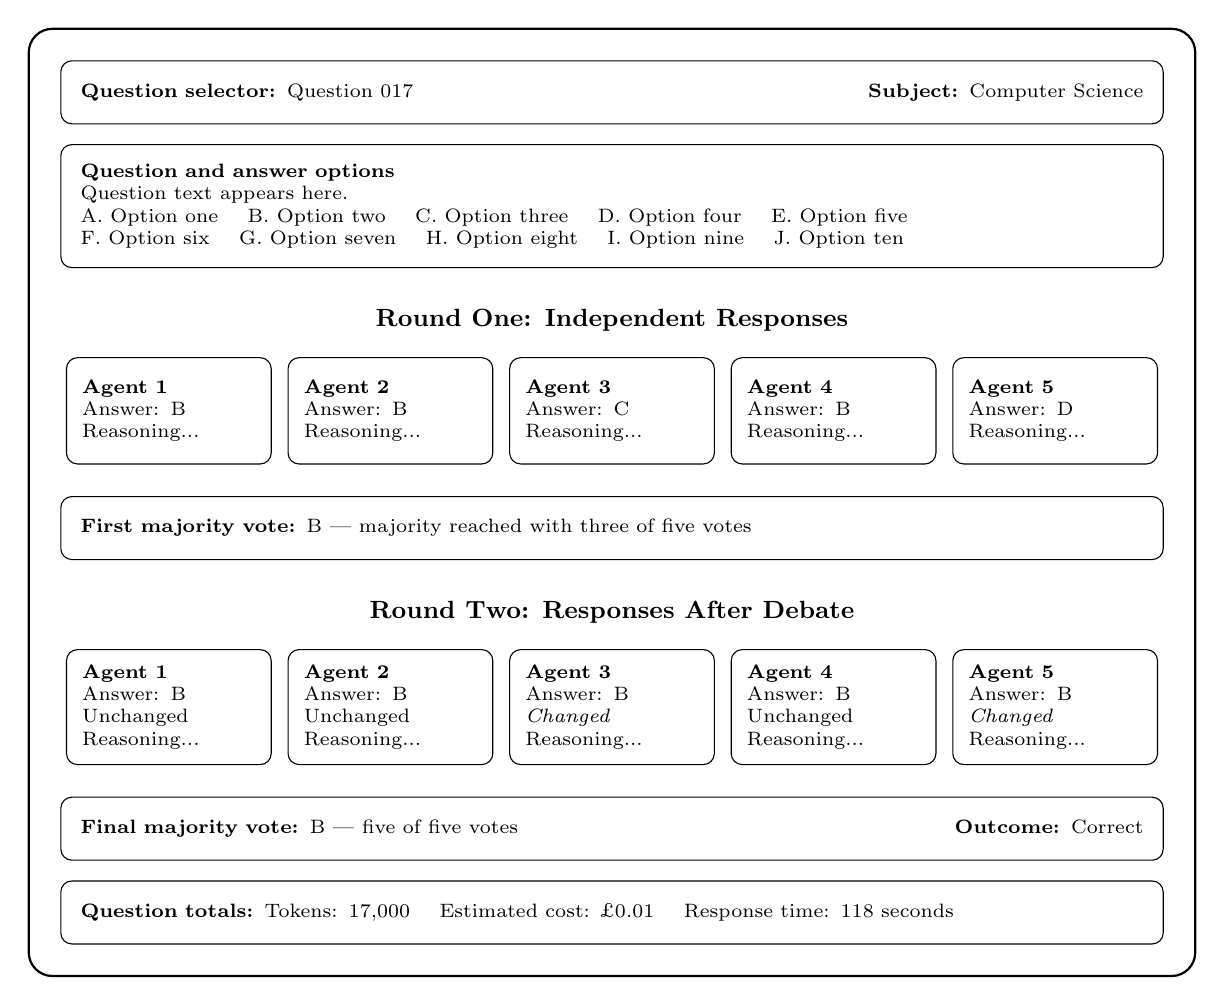
\begin{tikzpicture}[
        wide/.style={
            draw,
            rounded corners,
            align=left,
            text width=13.5cm,
            minimum height=0.8cm,
            inner sep=2.5mm,
            font=\scriptsize
        },
        agent/.style={
            draw,
            rounded corners,
            align=left,
            text width=2.2cm,
            minimum height=1.35cm,
            inner sep=2mm,
            font=\scriptsize
        },
        heading/.style={
            font=\small\bfseries
        },
        node distance=2.5mm
    ]

        \node[wide] (selector)
            {\textbf{Question selector:} Question 017
             \hfill
             \textbf{Subject:} Computer Science};

        \node[wide, below=of selector] (question)
            {\textbf{Question and answer options}\par
             Question text appears here.\par
             A. Option one \quad
             B. Option two \quad
             C. Option three \quad
             D. Option four \quad
             E. Option five\par
             F. Option six \quad
             G. Option seven \quad
             H. Option eight \quad
             I. Option nine \quad
             J. Option ten};

        \node[heading, below=4mm of question] (r1title)
            {Round One: Independent Responses};

        \node[agent, below=2mm of r1title] (r1a3)
            {\textbf{Agent 3}\par
             Answer: C\par
             Reasoning...};

        \node[agent, left=2mm of r1a3] (r1a2)
            {\textbf{Agent 2}\par
             Answer: B\par
             Reasoning...};

        \node[agent, left=2mm of r1a2] (r1a1)
            {\textbf{Agent 1}\par
             Answer: B\par
             Reasoning...};

        \node[agent, right=2mm of r1a3] (r1a4)
            {\textbf{Agent 4}\par
             Answer: B\par
             Reasoning...};

        \node[agent, right=2mm of r1a4] (r1a5)
            {\textbf{Agent 5}\par
             Answer: D\par
             Reasoning...};

        \node[wide, below=4mm of r1a3] (vote1)
            {\textbf{First majority vote:} B ---
             majority reached with three of five votes};

        \node[heading, below=4mm of vote1] (r2title)
            {Round Two: Responses After Debate};

        \node[agent, below=2mm of r2title] (r2a3)
            {\textbf{Agent 3}\par
             Answer: B\par
             \textit{Changed}\par
             Reasoning...};

        \node[agent, left=2mm of r2a3] (r2a2)
            {\textbf{Agent 2}\par
             Answer: B\par
             Unchanged\par
             Reasoning...};

        \node[agent, left=2mm of r2a2] (r2a1)
            {\textbf{Agent 1}\par
             Answer: B\par
             Unchanged\par
             Reasoning...};

        \node[agent, right=2mm of r2a3] (r2a4)
            {\textbf{Agent 4}\par
             Answer: B\par
             Unchanged\par
             Reasoning...};

        \node[agent, right=2mm of r2a4] (r2a5)
            {\textbf{Agent 5}\par
             Answer: B\par
             \textit{Changed}\par
             Reasoning...};

        \node[wide, below=4mm of r2a3] (final)
            {\textbf{Final majority vote:} B ---
             five of five votes
             \hfill
             \textbf{Outcome:} Correct};

        \node[wide, below=of final] (metrics)
            {\textbf{Question totals:}
             Tokens: 17,000 \quad
             Estimated cost: \pounds 0.01 \quad
             Response time: 118 seconds};

        \draw[thick, rounded corners=3mm]
            ([xshift=-4mm,yshift=4mm]selector.north west)
            rectangle
            ([xshift=4mm,yshift=-4mm]metrics.south east);

    \end{tikzpicture}%
    }
    
    \captionof{figure}{Initial design of the debate replay interface.}
    \label{fig:mockup}
\end{center}

\section{Project Ethics and Human Participants}
\label{sec:ethics}

As stated in Section~\ref{sec:ethical-compliance}, no human participants or
personal data are involved. OpenRouter receives benchmark questions and, in
round two, previous model responses with agent, model and provider identity
labels removed. API keys are kept in environment variables, and the replay
interface collects no user or participant data.

\section{BCS Project Criteria}
\label{sec:bcs}

\begin{enumerate}

    \item \textbf{Application of Practical and Analytical Skills}

    Building the system described in Section~\ref{sec:implementation} involves
    software design, API integration, result storage and automated tests. The
    analysis compares paired group votes on the same questions using accuracy,
    a confidence interval and a statistical test, alongside cost and time.

    \item \textbf{Innovation and Creativity}

    Many studies report only final group accuracy. This project measures each
    model, the first group vote and the vote after discussion, and tracks
    correct, incorrect and no-consensus transitions. This shows both whether
    accuracy changed and where the change occurred.

\end{enumerate}
% -------------------------------------------------
% Project plan
% -------------------------------------------------

\section{Project Plan}
\label{sec:plan}

The fixed milestones are the CA1 proposal on 11 September, the CA2 video on
6 November, the CA2 question-and-answer session between 9 and 13 November,
and the dissertation on 27 November. Figure~\ref{fig:gantt} shows the work
leading to them. The development periods are targets and will be reviewed
after the pilot, when the likely cost, running time and remaining work are
clearer. Week 1 begins on 3 August 2026.

\begin{center}
    \resizebox{0.65\textwidth}{!}{%
    \begin{ganttchart}[
        hgrid,
        vgrid,
        x unit=6.2mm,
        y unit title=5.0mm,
        y unit chart=4.5mm,
        title height=1,
        bar height=0.5,
        bar/.style={fill=black!25, draw=black!60},
        bar label font=\footnotesize,
        group label font=\footnotesize\bfseries,
        milestone label font=\footnotesize\itshape,
        title label font=\footnotesize,
        milestone/.style={fill=black, draw=black},
        progress label text={}
    ]{1}{17}

        \gantttitle{August}{4}
        \gantttitle{September}{4}
        \gantttitle{October}{5}
        \gantttitle{November}{4} \\

        \gantttitlelist{1,...,17}{1} \\

        \ganttgroup{Completed}{1}{4} \\
        \ganttbar{Literature review and design}{1}{3} \\
        \ganttbar{Dataset preparation and freezing}{2}{3} \\

        \ganttgroup{Proposal}{3}{6} \\
        \ganttbar{CA1 writing and checking}{3}{6} \\
        \ganttmilestone{CA1 submitted}{6} \\

        \ganttgroup{Implementation}{7}{11} \\
        \ganttbar{Limited project work}{7}{7} \\
        \ganttbar{Core components and round one}{8}{9} \\
        \ganttbar{Round-two runner}{10}{10} \\
        \ganttbar{Automated testing}{9}{10} \\
        \ganttbar{Evaluation script}{10}{11} \\

        \ganttgroup{Experiment}{11}{13} \\
        \ganttbar{Pilot, fixes and freeze}{11}{11} \\
        \ganttbar{Main run (300 questions)}{12}{12} \\
        \ganttbar{Results analysis}{12}{13} \\
        \ganttbar{Replay interface}{11}{13} \\

        \ganttgroup{Reporting}{8}{17} \\
        \ganttbar{Dissertation writing}{8}{16} \\
        \ganttbar{CA2 video}{13}{14} \\
        \ganttmilestone{CA2 submitted}{14} \\
        \ganttbar{Q\&A preparation}{15}{15} \\
        \ganttbar{Final checks and submission}{16}{17} \\
        \ganttmilestone{Dissertation submitted}{17}

    \end{ganttchart}%
    }
    
    \captionof{figure}{Project plan. Week 1 begins on 3 August 2026.}
    \label{fig:gantt}
\end{center}

The main experiment starts only after the pilot has passed and the prompts,
model settings, parsing rules and retry rules have been frozen. The evaluation
script will first be checked using the pilot results. The schedule leaves time
for API problems or a repeated run, while the replay interface will be ready
for the CA2 demonstration.



% -------------------------------------------------
% Risks and contingency plans
% -------------------------------------------------

\section{Risks and Contingency Plans}
\label{sec:risks}

The main risks to the project and the planned response to each are listed in
Table~\ref{tab:risks}.

\begin{table}[!htbp]
    \centering
    \footnotesize
    \renewcommand{\arraystretch}{1.1}

    \begin{tabularx}{\textwidth}{@{}LLll@{}}
        \toprule
        \textbf{Risk} &
        \textbf{Contingency} &
        \textbf{Likelihood} &
        \textbf{Impact} \\
        \midrule

        The correct answers are accidentally included in a model prompt &
        Answer keys are stored separately, and tests check prompts for leakage
        before the main experiment &
        Low &
        High \\

        \midrule

        API cost is higher than estimated &
        The pilot estimates cost per question, while the cache avoids paying
        twice for identical requests. Any change is discussed with the
        supervisor &
        Medium &
        High \\

        \midrule

        Round-two prompts exceed a model's context limit because they contain
        the agent's own previous response and up to four peer responses &
        The pilot checks context size. Prompt and response limits are then
        frozen before the main run &
        Medium &
        Medium \\

        \midrule

        One model refuses or returns unreadable answers too often to be usable &
        The pilot checks whether the problem is in the prompt, parser or model.
        Any replacement is agreed with the supervisor and tested again &
        Medium &
        High \\

        \midrule

        A pinned model or provider endpoint is withdrawn or changed &
        Exact model and provider identifiers are recorded, and automatic
        provider fallback is disabled. Any replacement is agreed with the
        supervisor and recorded as a new configuration &
        Low &
        High \\

        \midrule

        A pinned provider endpoint is unavailable or rate-limits requests &
        The same endpoint is retried once and persistent failures are recorded.
        The pilot will measure the failure rate, while the cache prevents
        completed calls from being purchased again &
        Medium &
        Medium \\

        \midrule

        Implementation takes longer than planned and delays the experiment &
        The schedule is reviewed each week. Desirable features and interface
        styling are delayed before essential work is changed &
        Medium &
        High \\

        \midrule

        Code, results or the frozen dataset are lost &
        Code and configuration are kept in version control. The results
        database and frozen dataset are backed up to separate storage after
        every run &
        Low &
        High \\

        \bottomrule
    \end{tabularx}

    \caption{Risk management plan.}
    \label{tab:risks}
\end{table}

\clearpage


\bibliographystyle{plainnat}
\bibliography{references}

\end{document}
